\section{Data preparation}
The dataset was built by extracting temporal data from the mp3 file provided in the file fma\_small.zip. The zip file contained 8,000 tracks with a duration of 30 seconds each. Each record was processed using the Librosa library, through which we extracted the time series using a sample rate of 8,000 (8 GHz). The latter guaranteed high quality tracks which are essential for performing our analysis. As the dimension and the storage-space required was exceptionally large (80,000 features and 14 GB of data), we decided to transform each audio wave into a time series of spectral centroid, which appeared to be more manageable and workable. We chose this feature transformation, as it is a well known measure used in digital signal processing to characterize a spectrum. During the extracting we detected few corrupted mp3 file which were discarded. In order to further reduce the size of our dataset, we filtered it down to 4 balanced genres: "Rock", "Hip-Hop", "Electronic" and "Experimental", for a total of 3994 time series with a length of 657 time stamps.
\begin{figure}[!htb]
  \centering
  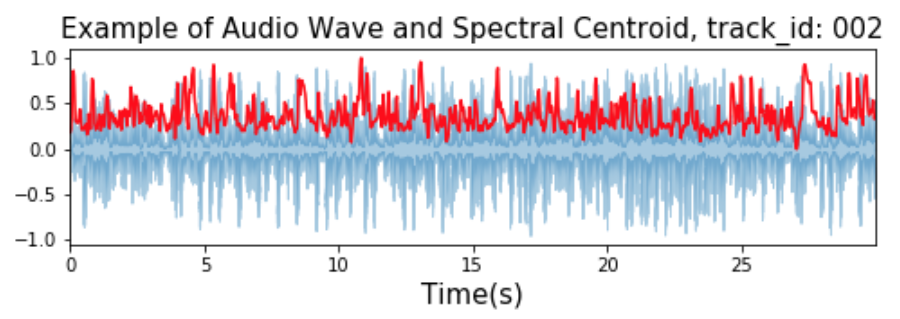
\includegraphics[width=0.5\linewidth]{images/spectralcentroid-audiowave-example.png}
  \caption{Audio wave (in blue) and Spectral Centroid (in red) for track\_id: 002.}
\end{figure}

\section{Time Series clustering: K-Means}

For this task we used the dataset described in the previous section. In the pre-processing step, since our aim was to focus on the shape of time-series, we first applied an amplitude scaling to improve their comparability, then we removed the noise by applying a moving average on a window = 3 time stamps. 
The chosen clustering algorithm (K-Means) was applied on the dataset approximated with SAX and PAA, as well as on the "raw" audio signal. The metrics we employed are the Euclidean and DTW. The last one, was tested using both Sakoe-Chiba band and Itakura parallelogram. 
After trying many configuration of segments' number and symbols' we selected 50 segments and 8 symbols (as they better approximeted the shape of the time series). We noticed that with very few segments the approximation resulted in a straight line. Instead as we increased the number of segments and symbols, the results didn't change in terms of shape. 
Below we show the approximation on one track as an illustrative example. 

\begin{figure}[!htb]
  \centering
  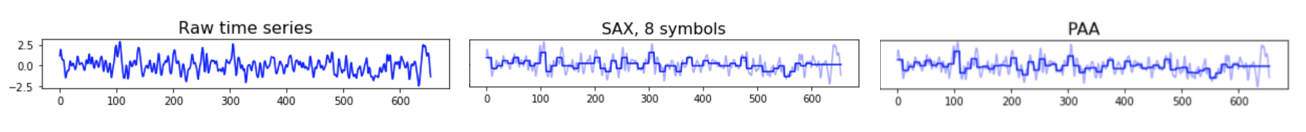
\includegraphics[width=1\linewidth]{images/example_SAX-PAA-RAW.png}
  \caption{Raw time series, SAX and PAA approximation on track 002.}
\end{figure}

The optimal number of clusters determined by computing the silhouette score and the SSE for every clustering (using a K in range 30). As it was not possible to determine the number of clusters by the "elbow-method", we decided to select the k that maximized the silhouette score. Independently from the approximation or distance, we noticed that the silhouette was approximately 0.05 for every clustering. This meant that the decision boundaries of each cluster were very close. After several trials, we selected k=4. The choice was driven by the fact that we were using a dataset that contained songs belonging to 4 different genres, therefore we wanted to see if K-Means was able to separate songs by genre, assigning them to their own cluster. 
We noticed that when we employed the euclidean distance, the composition of each cluster was homogeneous and no interesting results could be observed. This highlighted the fact that this distance metric was not suitable for time series, as misalignment caused substantial dissimilarities, even for those time series which were actually similar to one another. 
When we applied the DTW the clustering goodness improved. Results shown that although the Itakura parallelogram was generally inferior to the Sakoe-Chiba band, it was still superior to the unconstrained DTW. 
When using SAX and PAA approximation in combination with DTW, we were able to obtain an almost pure cluster for Hip-Hop songs. In fact in clusters where this genre represented the majority, we had very few Rock, Experimental and Electronic tracks. Furthermore, we noticed that in some clusters the composition of Rock and Electronic songs was very similar. After digging deeper in the reason for this grouping made by K-Means, we realized that some tracks of these 2 genres were very similar in terms of shape, probably due to the face that some rock tracks featured electronic instruments. 
Although the clustering performance improved when using SAX and PAA, the clustering on "raw" time series with the Sakoe-Chiba band DTW provided us the best results in terms of cluster composition.
In fact in Table 4.1 we can see (in yellow) that in each cluster there is a prevalence of each genre. It's interesting to notice that in cluster 2 and cluster 4, Hip-Hop songs are almost absent (with percentage not exceeding 0.5\%). Experimental and Rock songs have almost the same composition in cluster 4, whereas in cluster 2 we can observe a clear dominance of the former. Overall, if we observe the results obtained with the euclidean distance and DTW, we can conclude that the latter improved the performance and made each cluster more heterogeneous. 

\begin{figure}[!htb]
  \centering
  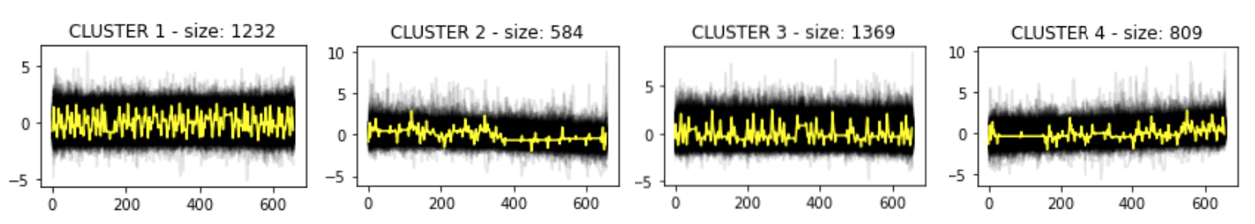
\includegraphics[width=1\linewidth]{images/centroids-DTW-RAW.png}
  \caption{Centroids of K-Means clustring on raw time series with DTW (Sakoe-Chiba band).}
\end{figure}

% Clusters of Raw TS - DTW

\begin{table}[htb]
\centering
\begin{tabular}{cccccc}
\hline
                   & \multicolumn{4}{c}{\textbf{Raw TS - DTW}}                                                                                                 &                           \\ \hline
\textbf{}          & \textbf{Hip-Hop}                 & \textbf{Rock}                    & \textbf{Electronic}              & \textbf{Experimental}            & \textit{\textbf{support}} \\ \hline
\textbf{Cluster 1} & 32.9 \%                          & 19.96 \%                         & \cellcolor[HTML]{FCFF2F}33.2 \%  & 13.79 \%                         & \textbf{1232}             \\ \hline
\textbf{Cluster 2} & 0.44 \%                          & 29.1 \%                          & 22.26 \%                         & \cellcolor[HTML]{FCFF2F}44.17 \% & \textbf{584}              \\ \hline
\textbf{Cluster 3} & \cellcolor[HTML]{FCFF2F}37.25 \% & 20.23 \%                         & 21.54 \%                         & 20.96 \%                         & \textbf{1369}             \\ \hline
\textbf{Cluster 4} & 0.06 \%                          & \cellcolor[HTML]{FCFF2F}37.82 \% & 20.27 \%                         & 35.10 \%                         & \textbf{809}              \\ \hline
                   & \multicolumn{4}{c}{\textbf{Raw TS - Euclidean}}                                                                                           &                           \\ \hline
\textbf{}          & \textbf{Hip-Hop}                 & \textbf{Rock}                    & \textbf{Electronic}              & \textbf{Experimental}            & \textit{\textbf{support}} \\ \hline
\textbf{Cluster 1} & 13.9 \%                          & 34.75 \%                         & \cellcolor[HTML]{FFFFFF}24.06 \% & 27.27 \%                         & \textbf{561}              \\ \hline
\textbf{Cluster 2} & 20.42 \%                         & 27.35 \%                         & 23.39 \%                         & \cellcolor[HTML]{FFFFFF}28.83 \% & \textbf{808}              \\ \hline
\textbf{Cluster 3} & \cellcolor[HTML]{FFFFFF}33.65 \% & 20.21 \%                         & 25.32 \%                         & 20.81 \%                         & \textbf{1994}             \\ \hline
\textbf{Cluster 4} & 13.15 \%                         & \cellcolor[HTML]{FFFFFF}28.52 \% & 26.94 \%                         & 31.37 \%                         & \textbf{631}              \\ \hline
\end{tabular}
 \caption{Clusters composition for K-Means with DTW and Euclidean ditance on the raw time series.}
\end{table}
\newpage
\section{Motifs and Anomaly Discovery}
In this section we extracted the top 10 motifs and top 5 anomalies from C-Doc's songs (42 tracks in total). In our dataset, this artist is one the principal exponents of the "Hip-Hop" genre.
Each motif was discovered using time series with a length of 657 time stamps (corresponding to 30 seconds) approximated with the spectral centroid. Before searching for patterns, we applied an amplitude scaling to each track. The matrix profile was then tested varying the size of the time window. In total we experimented with 15 configurations, trying low window values (i.e. 5) up to large values (i.e. 200). We noticed that the most accurate results were obtained with a window of 10. Similar patterns were observed in several C-Doc songs. Below we show only the most interesting results. 

\begin{figure}[!htb]
  \centering
  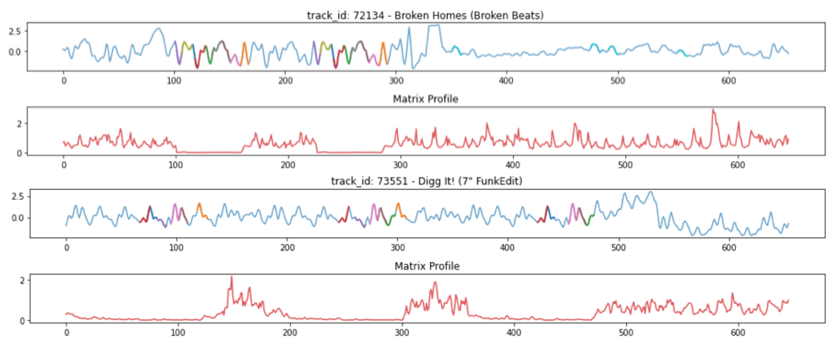
\includegraphics[width=0.9\linewidth]{images/CDOC-Motifs-MP.png}
  \caption{Motifs and Matrix Profile of C-Doc songs. "Broken Homes" and "Digg it!".}
\end{figure}

The Matrix Profile Index of the track "Broken Homes" shows motifs at index: [113, 238], [158, 283], [128, 253], [119, 244], [101, 226], [142, 267], [151, 276], [134, 259], [107, 232], [351, 476, 492, 554]. For those, the distances on the matrix profile (MP) are: [0.0040, 0.005, 0.005, 0.0071, 0.011, 0.013, 0.017, 0.0207, 0.0517, 0.245]. In figure 4.4, we can verify the presence of a repeating pattern starting from time stamp 100 up to 300.
In proximity of time stamps 580, we notice a spike in the matrix profile which corresponds to possible anomaly.
The song "Digg it!" instead, has a pattern repeating every 100 time stamps. Since the 30 seconds of each track were extracted from the central part of the song, it is intuitive to observe, that the motifs that emerged might be repetition of the melody in the main riff of the song. We also used the MP to detect discords in the time series. In order to detect anomalies, the exclusion zone was heuristically set to half of time window used in the MP (in this case the exclusion zone is 5). 
For simplicity, we show only few of them. The most evident discord of C-Doc tracks is in the song "Braggadocio" at time stamp 450. We can see a clearly see a peak in the spectrogram which is quite different from the overall pattern in the time series. In fact at that point the distance in the MP is the maximum.  
\begin{figure}[!htb]
  \centering
  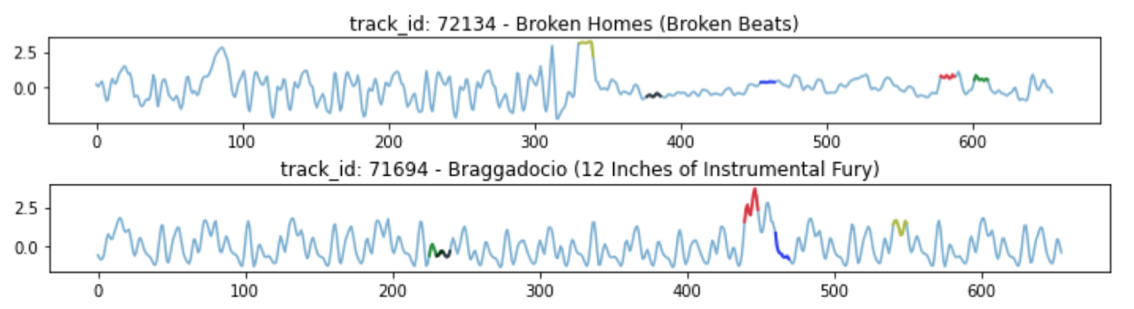
\includegraphics[width=0.8\linewidth]{images/CDOC - Anomalies.png}
  \caption{Anomalies in C-Doc songs: "Broken Homes" and "Braggadocio".}
\end{figure}

\section{Shapelet-based classification}

For this task we used the time series dataset described in the previous sections, filtered with only Hip-Hop and Rock songs as we wanted to solve a binary classification problem. The balanced dataset consisted of 1996 songs. To classify the genre, we built a KNN and a Decision tree using a dataset constructed using the top 5 shapelets.
We also evaluated the results of the classification, using different shapelets' number and lengths, however the highest performance was provided by 5 shapelets of length 56 (approximately 0.08\% of the time series length). Increasing the number of shapelets harmed the performance of our classifiers, with an accuracy that did not exceed 65\%. 
Before proceeding with the extraction, we split the data in training set (70\%) and test set (30\%). The shapelets were extracted exclusively from the training set. 
The model used for the shapelet-extraction was trained using Adam optimizer with a regularization of 0.01, over 1500 epochs. The validation accuracy obtained during the extraction resulted to be satisfactory (82,66 \% with a binary cross entropy of 0.4025). Below we show the 5 shapelets extracted, as well as their matching on 2 songs belonging to different genres, which were correctly classified on the test set. We observed that although the shapelets appeared very dissimilar from the motifs extracted for the Hip-Hop artist "C-Doc", we noticed a slight correlation in terms of shape between shapelet 4 and the motifs of the track "Broken Homes" (Figure 4.4). 

\begin{figure}[!htb]
  \centering
  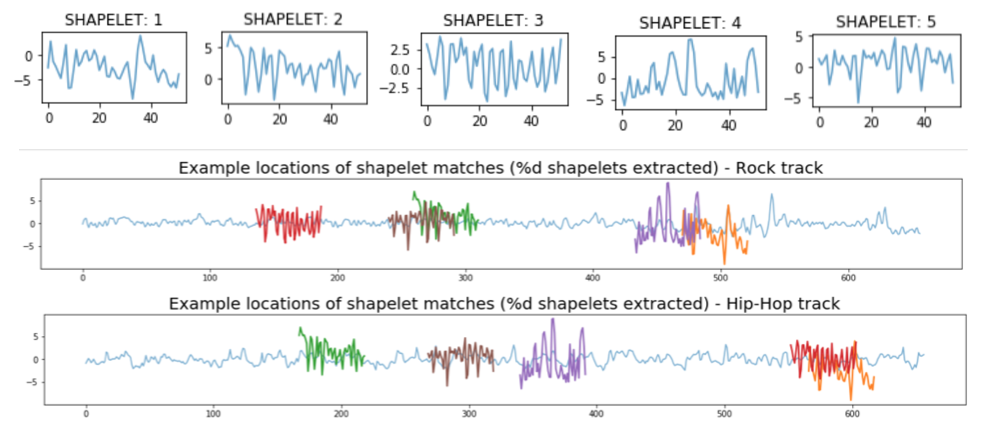
\includegraphics[width=0.85\linewidth]{images/shapelets.png}
  \caption{Example of matching between Rock and Hip-Hop time series with the extracted shapelets.}
\end{figure}

After we constructed the shapelet-based dataset, we used it to train a KNN and a decision tree classifier. The hyper-parameters of each model were fine-tuned through a coarse grid search and a 5 fold cross validation. The best accuracy was yielded by the KNN with K=23 in combination with the Manhattan distance. As we can see from Table 4.2, the KNN outperformed the decision tree, with an increment in the accuracy of approximately 4\%.


\begin{table}[ht]
\begin{tabular}{
>{\columncolor[HTML]{FFFFFF}}c 
>{\columncolor[HTML]{FFFFFF}}c 
>{\columncolor[HTML]{FFFFFF}}c 
>{\columncolor[HTML]{FFFFFF}}c l
>{\columncolor[HTML]{FFFFFF}}l 
>{\columncolor[HTML]{FFFFFF}}l 
>{\columncolor[HTML]{FFFFFF}}l 
>{\columncolor[HTML]{FFFFFF}}l }
\cline{1-4} \cline{6-9}
                  & \multicolumn{3}{c}{\cellcolor[HTML]{FFFFFF}\textbf{Shapelet-based KNN}} &  & \multicolumn{3}{c}{\cellcolor[HTML]{FFFFFF}\textbf{Shapelet-based Decision Tree}} &                  \\ \cline{1-4} \cline{6-9} 
\textbf{}         & \textbf{Precision}      & \textbf{Recall}      & \textbf{f1-score}      &  & \textbf{Precision}          & \textbf{Recall}         & \textbf{f1-score}         & \textbf{Support} \\ \cline{1-4} \cline{6-9} 
\textbf{Hip-Hop}  & 80\%                    & 73\%                 & 76\%                   &  & 76\%                        & 67\%                    & 71\%                      & 299              \\ \cline{1-4} \cline{6-9} 
\textbf{Rock}     & 75\%                    & 82\%                 & 79\%                   &  & 71\%                        & 79\%                    & 75\%                      & 300              \\ \cline{1-4} \cline{6-9} 
\textbf{Accuracy} & \multicolumn{3}{c}{\cellcolor[HTML]{FFFFFF}77.62 \%}                    &  & \multicolumn{4}{c}{\cellcolor[HTML]{FFFFFF}73.12 \%}                                                 \\ \cline{1-4} \cline{6-9} 
\end{tabular}
\caption{Calssification report of shapelet classifiers. KNN: n\_neigh=23, metric = Manhattan.\\ Decision Tree: max\_depth = 12, min\_sample\_leaf = 8, min\_sample\_split = 2, criterion = Entropy.}
\end{table}

